% file: binom-4-2.tex

\documentclass{standalone}
\usepackage{tikz}
\usepackage{tikz-qtree}
\usetikzlibrary{shapes}

\begin{document}
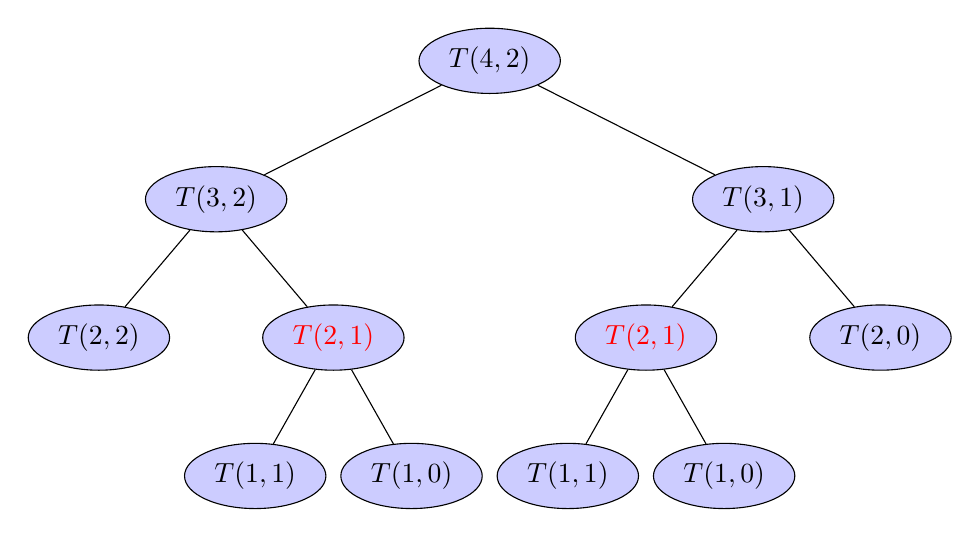
\begin{tikzpicture}[level distance = 50pt, sibling distance = 5pt,
  edge from parent/.style= { % added code
      draw, edge from parent path = {(\tikzparentnode) -- (\tikzchildnode)}},
    leaf/.style = {rectangle, rounded corners, fill = lightgray!40}]
  \tikzset{every tree node/.style = 
    {align = center, ellipse, draw, fill = blue!20}}

    \Tree [.{$T(4,2)$}	
      		[.{$T(3,2)$} 
		  [.{$T(2,2)$} ] 
		  [.{\textcolor{red}{$T(2,1)$}} 
		    [.{$T(1,1)$} ]
		    [.{$T(1,0)$} ]
		  ]
               ]
	       [.{$T(3,1)$} 
		 [.{\textcolor{red}{$T(2,1)$}}
		    [.{$T(1,1)$} ]
		    [.{$T(1,0)$} ]
		 ] 
		 [.{$T(2,0)$} ]
	       ]
	]
  \end{tikzpicture}
\end{document}